\documentclass[tikz,border=10pt]{standalone}
\usetikzlibrary{positioning, arrows.meta, calc, shapes.geometric, babel, fit, backgrounds}
\usepackage[utf8]{inputenc}
\usepackage[T1]{fontenc}
\usepackage{lmodern}
\usepackage[english]{babel}
\usepackage{amsmath, amssymb, bm}

\begin{document}
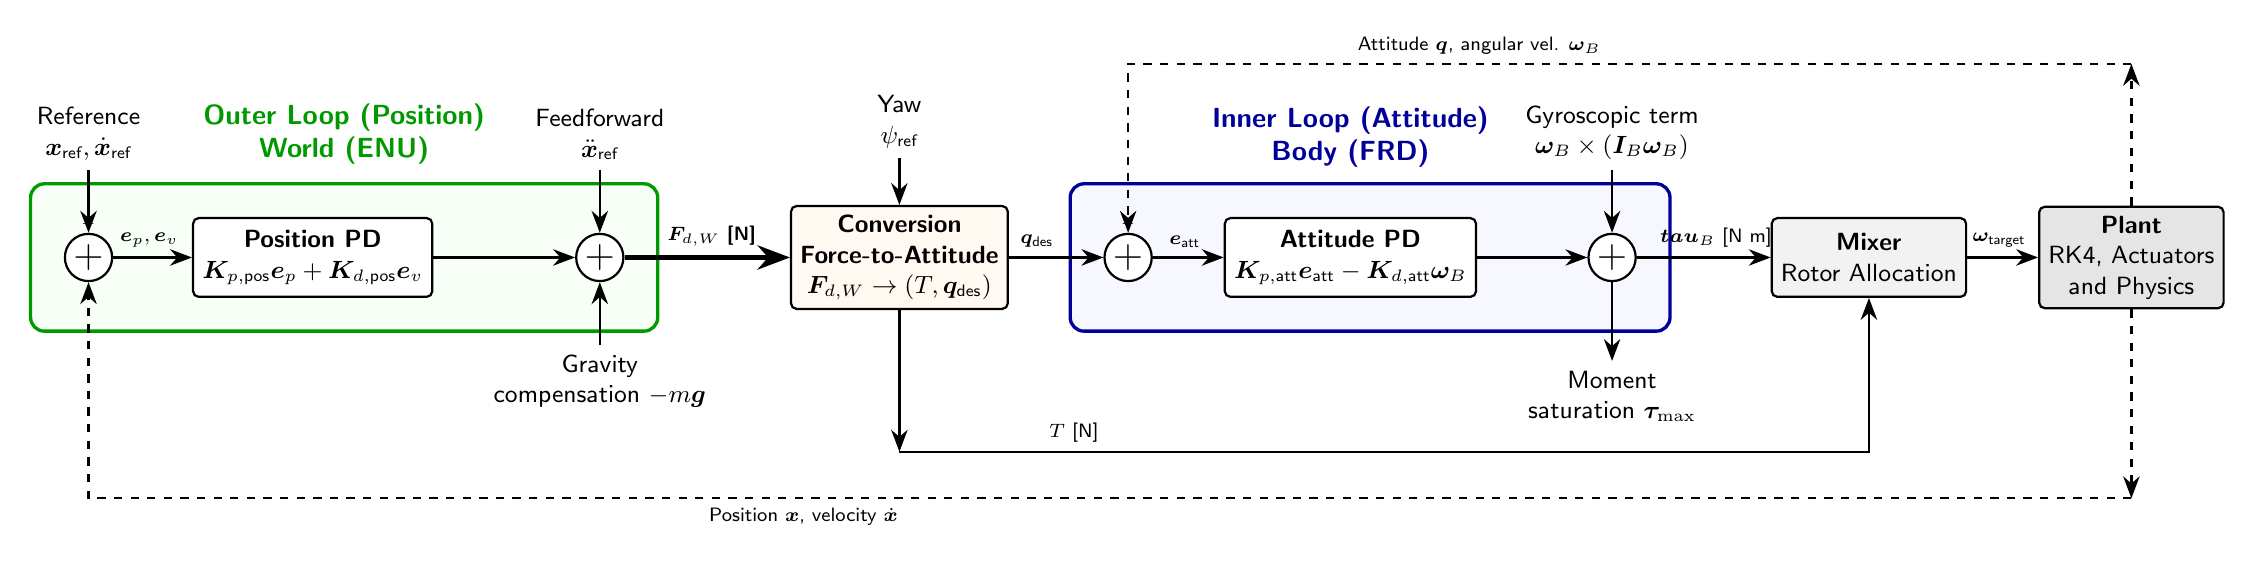
\begin{tikzpicture}[
  node distance=0.8cm and 1.6cm,
  align=center,
  font=\sffamily\small,
  % Estilos de bloques
  box/.style={draw, rectangle, rounded corners=2pt, minimum width=2.2cm, minimum height=1.0cm, thick, fill=white},
  sum/.style={draw, circle, minimum size=0.6cm, thick, fill=white, inner sep=0pt},
  groupbox/.style={draw, rectangle, rounded corners=5pt, line width=1.2pt, inner sep=12pt},
  % Estilos de flechas
  line/.style={draw, -{Stealth[scale=1.2]}, thick},
  dashline/.style={draw, -{Stealth[scale=1.2]}, thick, dashed}
]

  % Coordenada de inicio
  \coordinate (start) at (0,0);

  % ==========================================
  % OUTER LOOP: POSITION (ENU / WORLD)
  % ==========================================
  \node[sum] (sum_pos) at (start) {\Large $+$};
  \node[anchor=south west, font=\sffamily\tiny] at (sum_pos.north west) {$-$};
  
  \node[box, right=1 cm of sum_pos] (pd_pos) {
    \textbf{Position PD}\\
    $\bm{K}_{p,\text{pos}} \bm{e}_p + \bm{K}_{d,\text{pos}} \bm{e}_v$
  };
  
  \node[sum, right=1.8cm of pd_pos] (sum_acc) {\Large $+$};
  
  % Conectar
  \draw[line] (sum_pos) -- node[above, font=\sffamily\scriptsize] {$\bm{e}_p, \bm{e}_v$} (pd_pos);
  \draw[line] (pd_pos) -- (sum_acc);
  
  % Entradas de prealimentación externas
  \node[above=0.8cm of sum_pos] (ref_pos) {Reference\\$\bm{x}_{\text{ref}}, \dot{\bm{x}}_{\text{ref}}$};
  \node[above=0.8cm of sum_acc] (ref_acc) {Feedforward\\$\ddot{\bm{x}}_{\text{ref}}$};
  \node[below=0.8cm of sum_acc] (g_comp) {Gravity\\compensation $-m\bm{g}$};
  
  \draw[line] (ref_pos.south) -| (sum_pos.north);
  \draw[line] (ref_acc.south) -- (sum_acc.north);
  \draw[line] (g_comp.north) -- (sum_acc.south);

  % ==========================================
  % FORCE-TO-ATTITUDE CONVERSION
  % ==========================================
  \node[box, right=2.1cm of sum_acc, fill=orange!5, minimum width=2.4cm] (conversion) {
    \textbf{Conversion}\\
    \textbf{Force-to-Attitude}\\
    $\bm{F}_{d,W} \to (T, \bm{q}_{\text{des}})$
  };
  
  \draw[line, line width=1.5pt] (sum_acc.east) -- node[above, xshift=0.1cm, font=\sffamily\bfseries\scriptsize] {$\bm{F}_{d,W}$ [N]} (conversion.west);

  % Entrada de guiñada de referencia a la conversión
  \node[above=0.6cm of conversion] (ref_guiñada) {Yaw\\$\psi_{\text{ref}}$};
  \draw[line] (ref_guiñada) -- (conversion);

  % ==========================================
  % INNER LOOP: ATTITUDE (FRD / BODY)
  % ==========================================
  \node[sum, right=1.2cm of conversion] (sum_att) {\Large $+$};
  \node[anchor=south west, font=\sffamily\tiny] at (sum_att.north west) {$-$};

  \node[box, right=0.9cm of sum_att] (pd_att) {
    \textbf{Attitude PD}\\
    $\bm{K}_{p,\text{att}} \bm{e}_{\text{att}} - \bm{K}_{d,\text{att}} \bm{\omega}_B$
  };
  
  \node[sum, right=1.4cm of pd_att] (sum_gyro) {\Large $+$};

  % Conexiones internas
  \draw[line] (sum_att) -- node[above, font=\sffamily\scriptsize] {$\bm{e}_{\text{att}}$} (pd_att);
  \draw[line] (pd_att) -- (sum_gyro);

  \node[above=0.8cm of sum_gyro] (gyro) {Gyroscopic term\\$\bm{\omega}_B \times (\bm{I}_B \bm{\omega}_B)$};
  \node[below=1.0 cm of sum_gyro] (sat_mom) {Moment\\saturation $\bm{\tau}_{\max}$};

  \draw[line] (gyro) -- (sum_gyro.north);
  \draw[line] (sum_gyro.south) -- (sat_mom.north);

  % ==========================================
  % CONTEXT GROUPS
  % ==========================================
  \begin{scope}[on background layer]
    % Contenedor Lazo Externo
    \node[groupbox, draw=green!60!black, fill=green!3, fit=(sum_pos) (pd_pos) (sum_acc)] (externo_group) {};
    
    % Contenedor Lazo Interno
    \node[groupbox, draw=blue!60!black, fill=blue!3, fit=(sum_att) (pd_att) (sum_gyro)] (interno_group) {};
  \end{scope}

  \node[anchor=south, font=\sffamily\bfseries, color=green!60!black, align=center] at ($(externo_group.north) + (0,0.1)$) {Outer Loop (Position)\\World (ENU)};
  \node[anchor=south, font=\sffamily\bfseries, color=blue!60!black, align=center] at ($(pd_att.north) + (0,0.5)$) {Inner Loop (Attitude)\\Body (FRD)};

  % Conexiones de la conversión al lazo interno
  \draw[line] (conversion.east) -- node[above, xshift=-0.2cm, font=\sffamily\scriptsize] {$\bm{q}_{\text{des}}$} (sum_att.west);

  % ==========================================
  % MIXER AND PLANT
  % ==========================================
  \node[box, right=1.7cm of sum_gyro, fill=gray!10] (mixer) {
    \textbf{Mixer}\\
    Rotor Allocation
  };
  
  \node[box, right=0.9cm of mixer, fill=gray!20] (planta) {
    \textbf{Plant}\\
    RK4, Actuators\\
    and Physics
  };

  % Conectar lazo interno al mixer
  \draw[line] (sum_gyro.east) -- node[above, xshift=0.2cm, font=\sffamily\scriptsize] {$\bm{tau}_B$ [N m]} (mixer.west);
  
  % Empuje colectivo
  \coordinate (t_corner) at ($(conversion.south) + (0,-1.8)$);
  \draw[line] (conversion.south) -- (t_corner);
  \draw[line] (t_corner) -| (mixer.south);
  \node[above, font=\sffamily\scriptsize] at ($(t_corner)!0.18!(mixer.south |- t_corner)$) {$T$ [N]};

  % Conexión directa mixer -> planta
  \draw[line] (mixer.east) -- node[above, font=\sffamily\scriptsize] {$\bm{\omega}_{\text{target}}$} (planta.west);

  % ==========================================
  % FEEDBACK PATHS
  % ==========================================
  
  % 1. Attitude feedback (Inner loop)
  \draw[dashline] (planta.north) -- ++(0, 1.8) coordinate (fb_att_h);
  \draw[dashline] (fb_att_h) -| (sum_att.north);
  \node[above, font=\sffamily\scriptsize] at ($(fb_att_h)!0.65!(sum_att.north |- fb_att_h)$)
    {Attitude $\bm{q}$, angular vel. $\bm{\omega}_B$};

  % 2. Position feedback (Outer loop)
  \draw[dashline] (planta.south) -- ++(0, -2.4) coordinate (fb_pos_h);
  \draw[dashline] (fb_pos_h) -| (sum_pos.south);
  \node[below, font=\sffamily\scriptsize] at ($(fb_pos_h)!0.65!(sum_pos.south |- fb_pos_h)$)
    {Position $\bm{x}$, velocity $\dot{\bm{x}}$};

\end{tikzpicture}
\end{document}
